\section{Empirical}

%%%%%%%%%%%%%%%%%%%%%%%%%%%%%%%%%%%%%%%%%%%%%%%%%%%%%%%%%%%%%%%%%%%%%%%%%%
\begin{table*}[tbp!]
\centering
\begin{tabular}{|l|r|r|r|r|l|} \hline
Dataset & \# Features & \# Data & \# Features/\# Data & \% True Labels & Feature Type\\ \hline \hline 
Breast Cancer	& 9	& 699	& 0.013	& 34 \%	& All Numeric\\ \hline
Diabetes        & 8	& 768	& 0.010	& 35 \%	& All Numeric\\ \hline
Heart Statlog	& 13	& 270	& 0.048	& 44 \%	& All Numeric\\ \hline
Spect	        & 22	& 80	& 0.275 & 33 \%	& Categorical\\ \hline
Vote	        & 16	& 435	& 0.037	& 39 \%	& Categorical\\ \hline
Newsgroup	& 500	& 1963	& 0.255	& 49 \%	& All Binary\\ \hline
Horse Colic	& 22	& 368	& 0.060	& 37 \%	& Categorical (16) and numeric (6)\\ \hline
Credit-American	& 15	& 690	& 0.022	& 44 \%	& Categorical(9) and numeric (6)\\ \hline
Credit-German	& 20	& 1000	& 0.020 & 30 \%	& Categorical (13) and Numeric (7)\\ \hline
Hepatitis	& 19	& 155	& 0.123	& 21 \%	& Categorical (13) and Numeric (6)\\ \hline
Ionosphere	& 34	& 351	& 0.097	& 36 \%	& All Numeric\\ \hline
%KR-vs-KP	& 36	& 3196	& 0.011	& 48 \%	& All Categorical\\ \hline
%Labor	        & 16	& 57	& 0.281	& 35 \%	& Categorical (8) and Numeric (8)\\ \hline
%Mushroom	& 22	& 8124	& 0.003	& 48 \%	& All Categorical\\ \hline
%Sick	        & 29	& 3772	& 0.008	&  6 \%	& Categorical (23) and Numeric (6)\\ \hline
%Sonar	        & 60	& 208	& 0.288 & 47 \%	& All Numeric\\ \hline
\end{tabular}
\caption{\footnotesize Statistics of the various datasets evaluated in this work.}
\label{table:stats}
\end{table*}
%%%%%%%%%%%%%%%%%%%%%%%%%%%%%%%%%%%%%%%%%%%%%%%%%%%%%%%%%%%%%%%%%%%%%%%%%%

In this section, we conduct experiments to study the feature selection
performances of several well known methods such as Symmetrical
Uncertainty Rank (SUR), Gain Ratio Rank (GRR), Information Gain Rank
(IGR), Correlation Based Rank (CBR), Conditional Entropy Rank (CER)~\cite{guyon_jmlr03}, 
Correlation-based Feature Subset Selection (CFS)~\cite{Hall1998}, 
Reliff (R)~\cite{Robnik-Sikonja2003} , mRMR~\cite{peng2005} and our proposed 
methods: High Recall Expectation (HRE) and High Recall Log likelihood (HRL), 
High Precision Expectation (HPE), High Precision Log likelihood (HPL). 
The first five methods are variable rank methods and the last seven
are subset rank methods. The first five methods are variable rank methods that select variables by ranking them with some metric and the last seven are subset rank methods that assess subsets of variables and consider previous selections to decide the next selection.

{\bf TODO Rodrigo: please update acronyms in plots with those given above,
use MRMR for MRMR... sorry, does not seem sensible to shorten this to 3 letters.}

% TODO: Scott... any interesting things to point out?  
%       Class imbalance / feature-data ratios?

In this experimental study, we evaluated each feature selection
method on a variety of binary classification problems 
from the UCI machine learning repository \cite{Bache+Lichman:2013}.
These datasets along with their properties are outlined in 
Table~\ref{table:stats}.

In addition, we used three different classifiers to solve each of the
binary classifier problem. Logistic Regression (LR), SVM Linear (SVM) and Naive
Bayes (NB) were used in the experiments and the first two are implemented
in the LibLinear library~\cite{REF08a} and the last one is implemented in
the Weka software~\cite{weka}.
 
To evaluate feature selection algorithm performance, we perform 
10-fold nested cross-validation (nesting for tuning hyperparameters of each classification
algorithm) and evaluate accuracy, precision, and recall at each stage of
feature selection from the first selected feature through to the maximum
(either 50 or the number of features in the dataset, whichever is smaller).
%and F-Score for the true label class, that
%could be identified by the context of the problem and usually be the
%class with least samples in the data set.

In our evaluation, we wish to answer the following questions:
Do different feature selection methods perform better with
each classifier or on each dataset in comparison to others?
How reliably do the different feature selection methods perform overall
in terms of their performance distribution?
%\item Do any dataset features seem to correlate with algorithm performance?

%%%%%%%%%%%%%%%%%%%%%%%%%%%%%%%%%%%%%%%%%%%%%%%%%%%%%%%%%%%%%%%%%%%%%%%%%%
\begin{figure*}[tbp!]
\centering
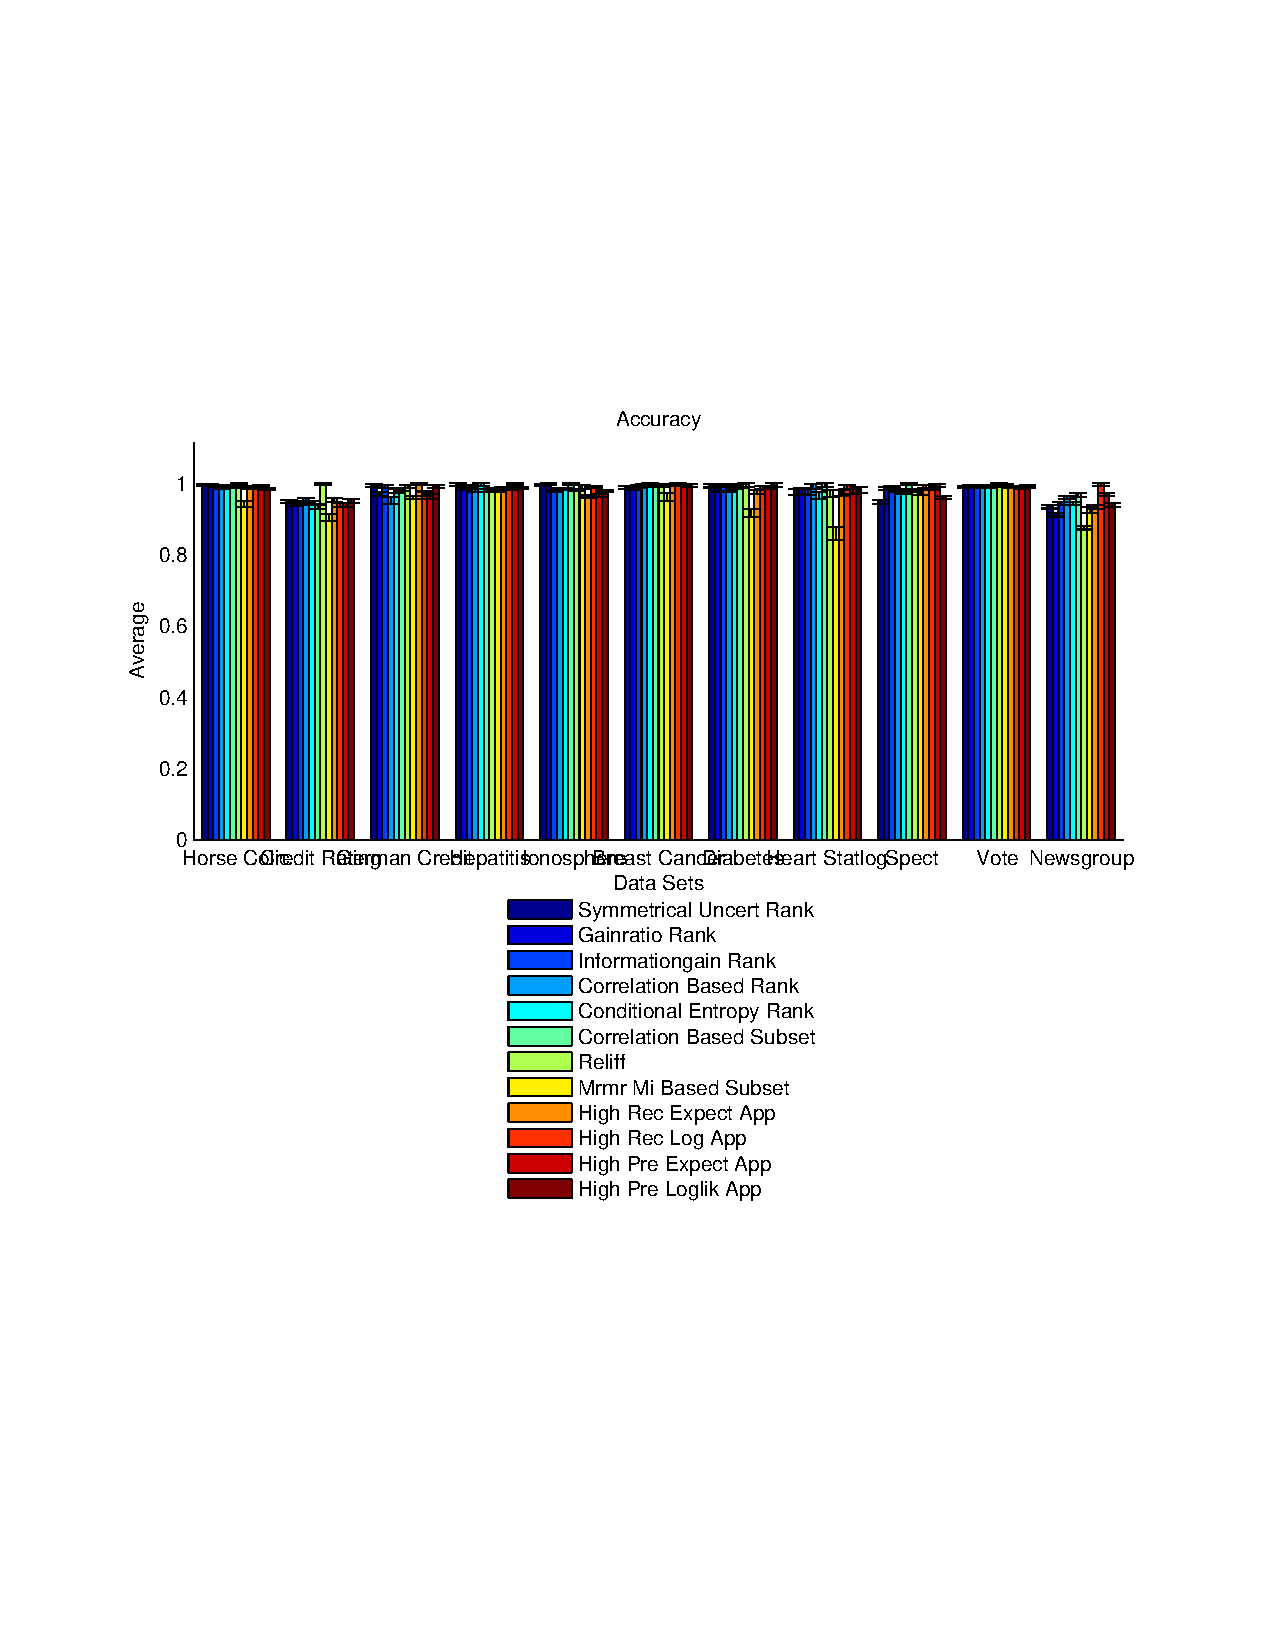
\includegraphics[width=0.35\textwidth]{../ResultsPlot/OthersDataSets/BarGraphs/dataSetXFeatureSelection_avgCl/Accuracy.pdf}\\
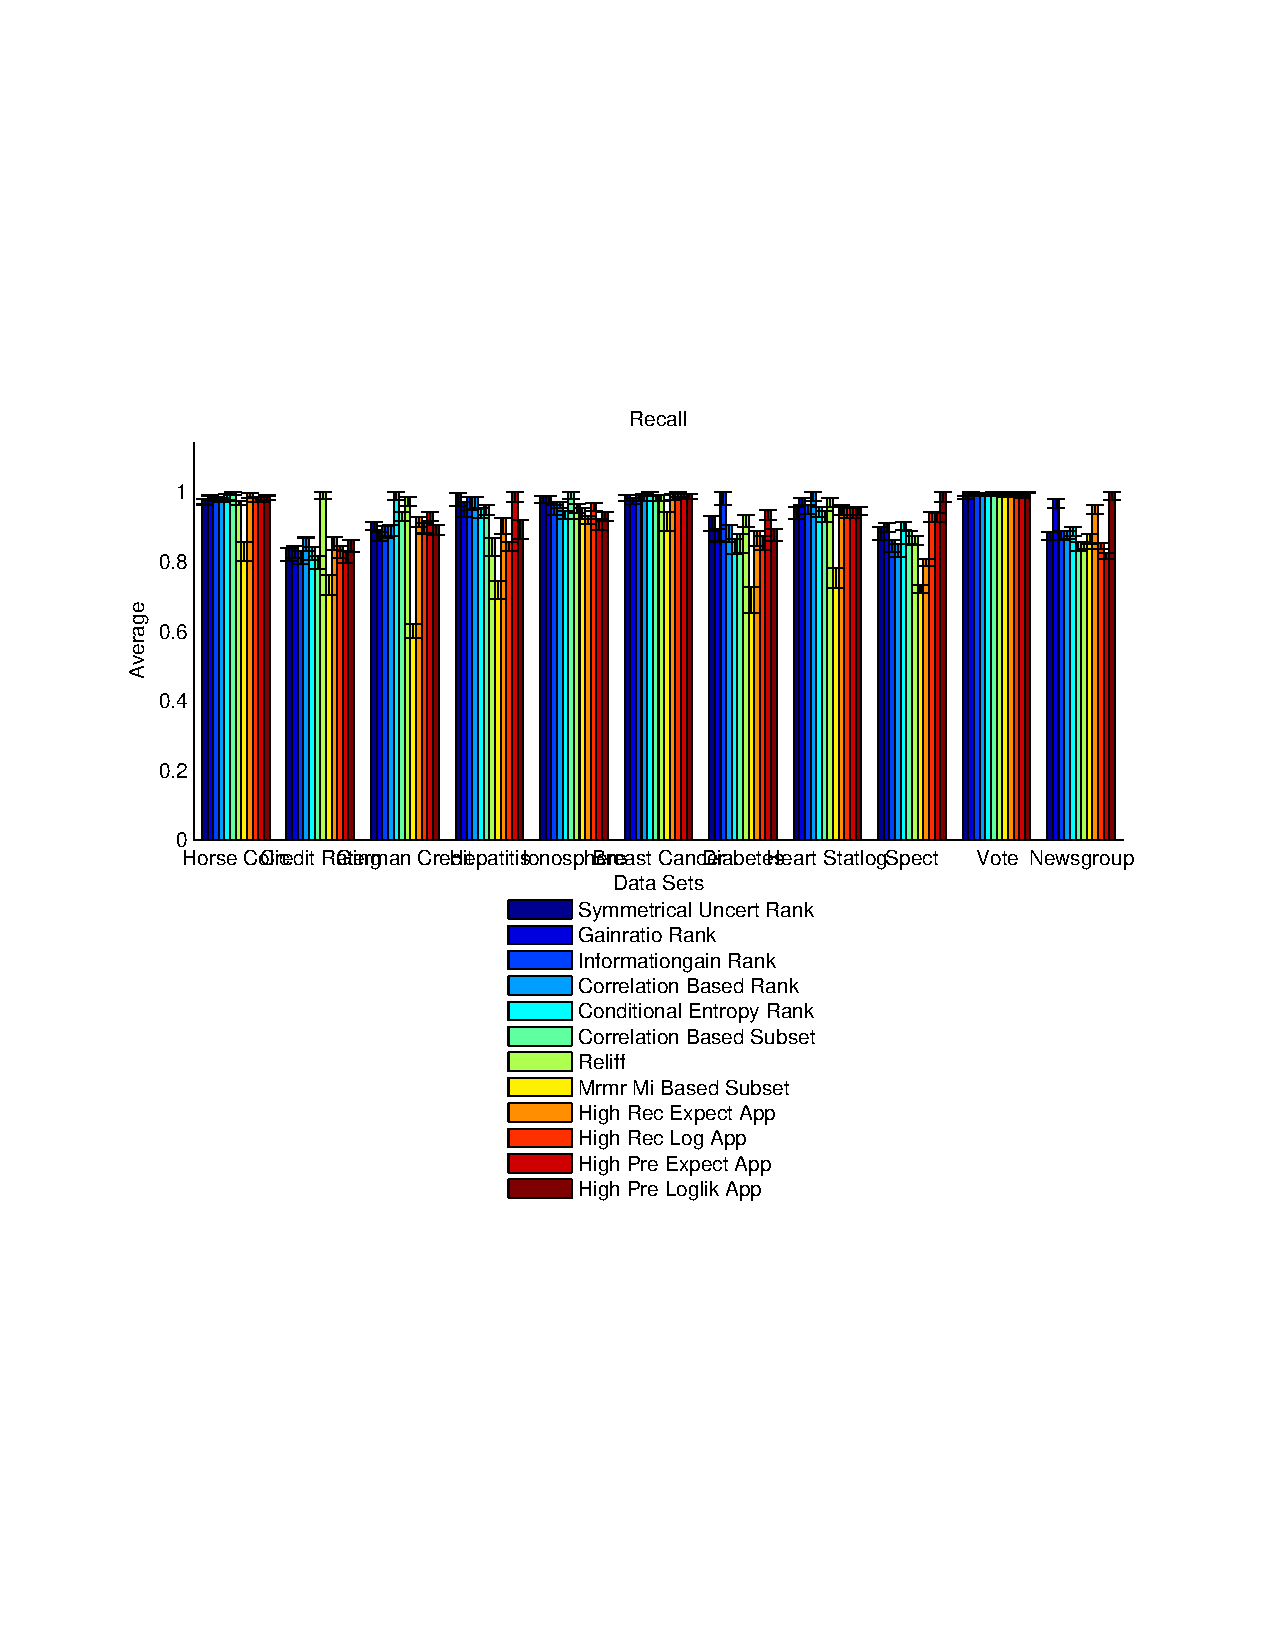
\includegraphics[width=0.35\textwidth]{../ResultsPlot/OthersDataSets/BarGraphs/dataSetXFeatureSelection_avgCl/Recall.pdf}
\caption{\footnotesize Performance of various feature selection algorithms per dataset, averaged across classifier type and each stage of feature selection.}
\label{fig:perf_vs_dataset}
\end{figure*}
%%%%%%%%%%%%%%%%%%%%%%%%%%%%%%%%%%%%%%%%%%%%%%%%%%%%%%%%%%%%%%%%%%%%%%%%%%

%%%%%%%%%%%%%%%%%%%%%%%%%%%%%%%%%%%%%%%%%%%%%%%%%%%%%%%%%%%%%%%%%%%%%%%%%%
\begin{figure*}[tbp!]
\centering
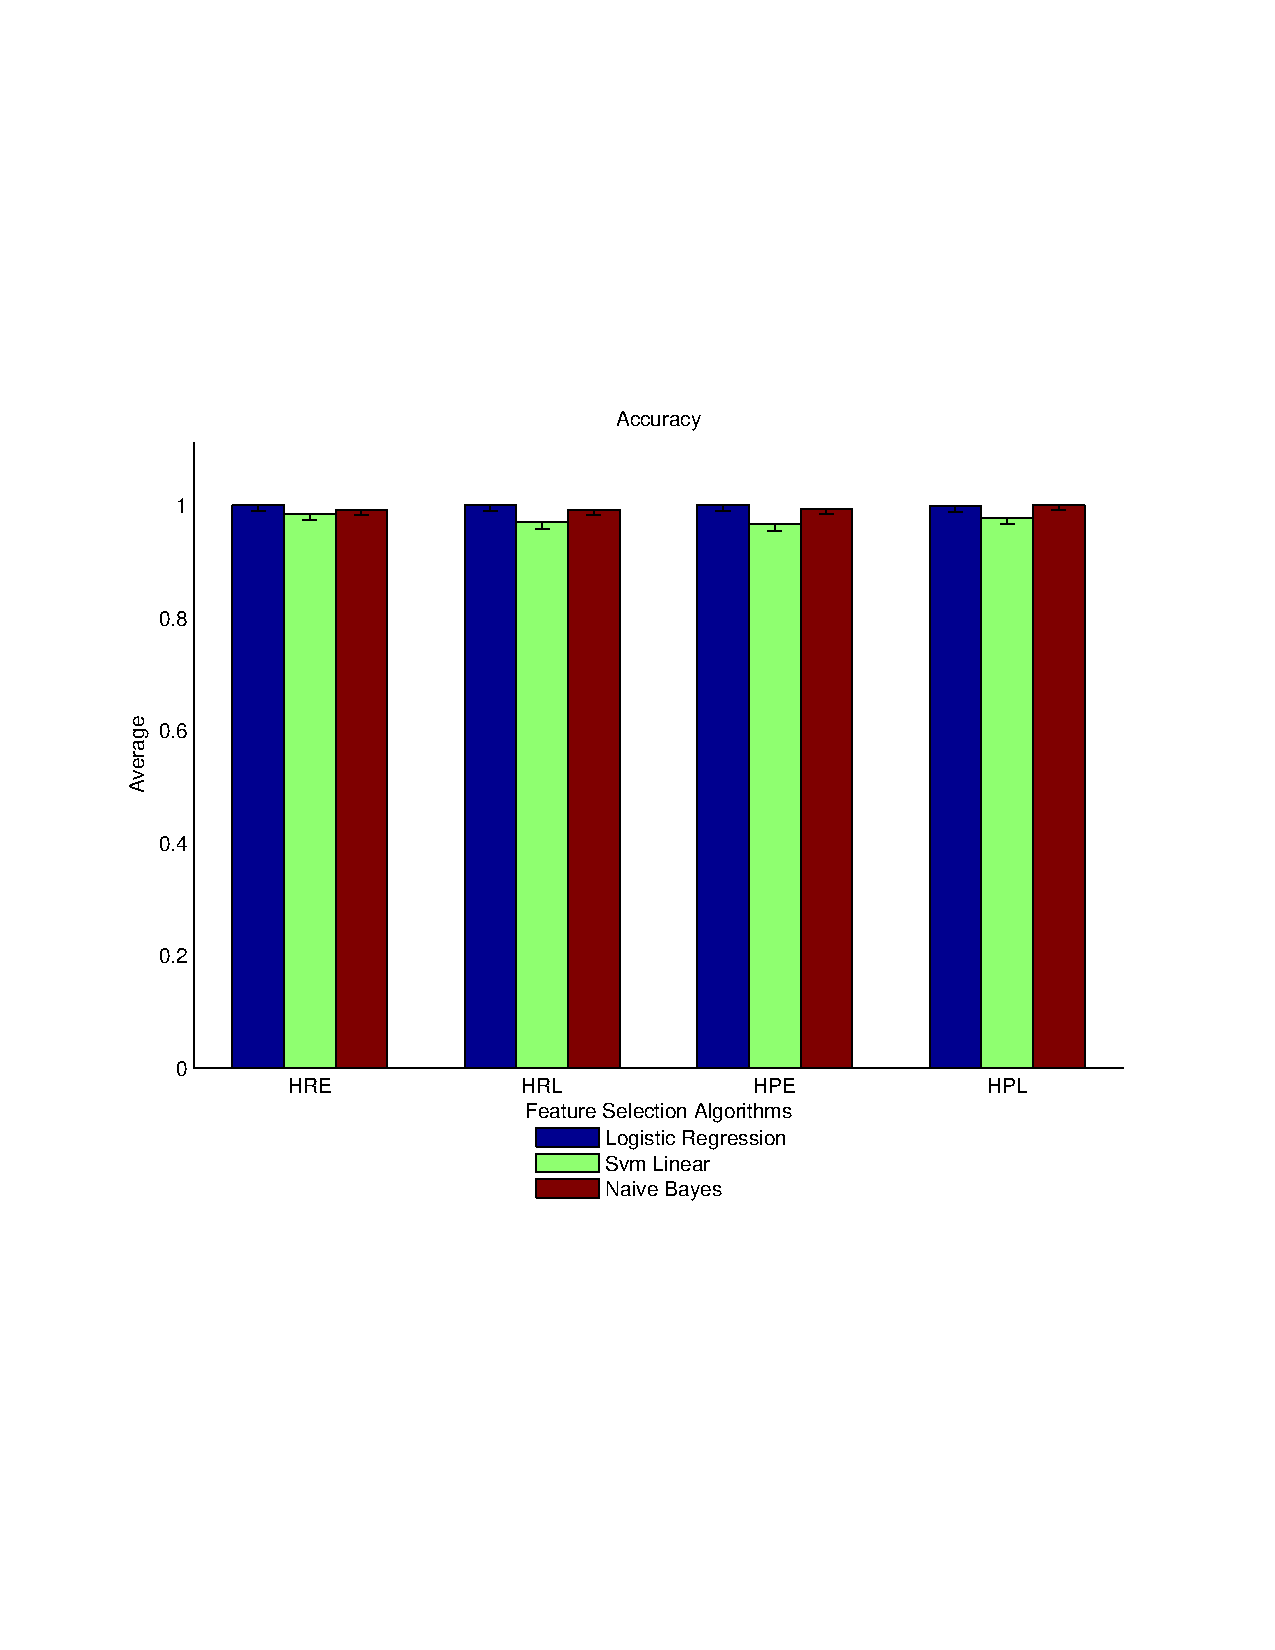
\includegraphics[width=0.35\textwidth]{../ResultsPlot/OthersDataSets/BarGraphs/bargraph4/Accuracy.pdf}\\
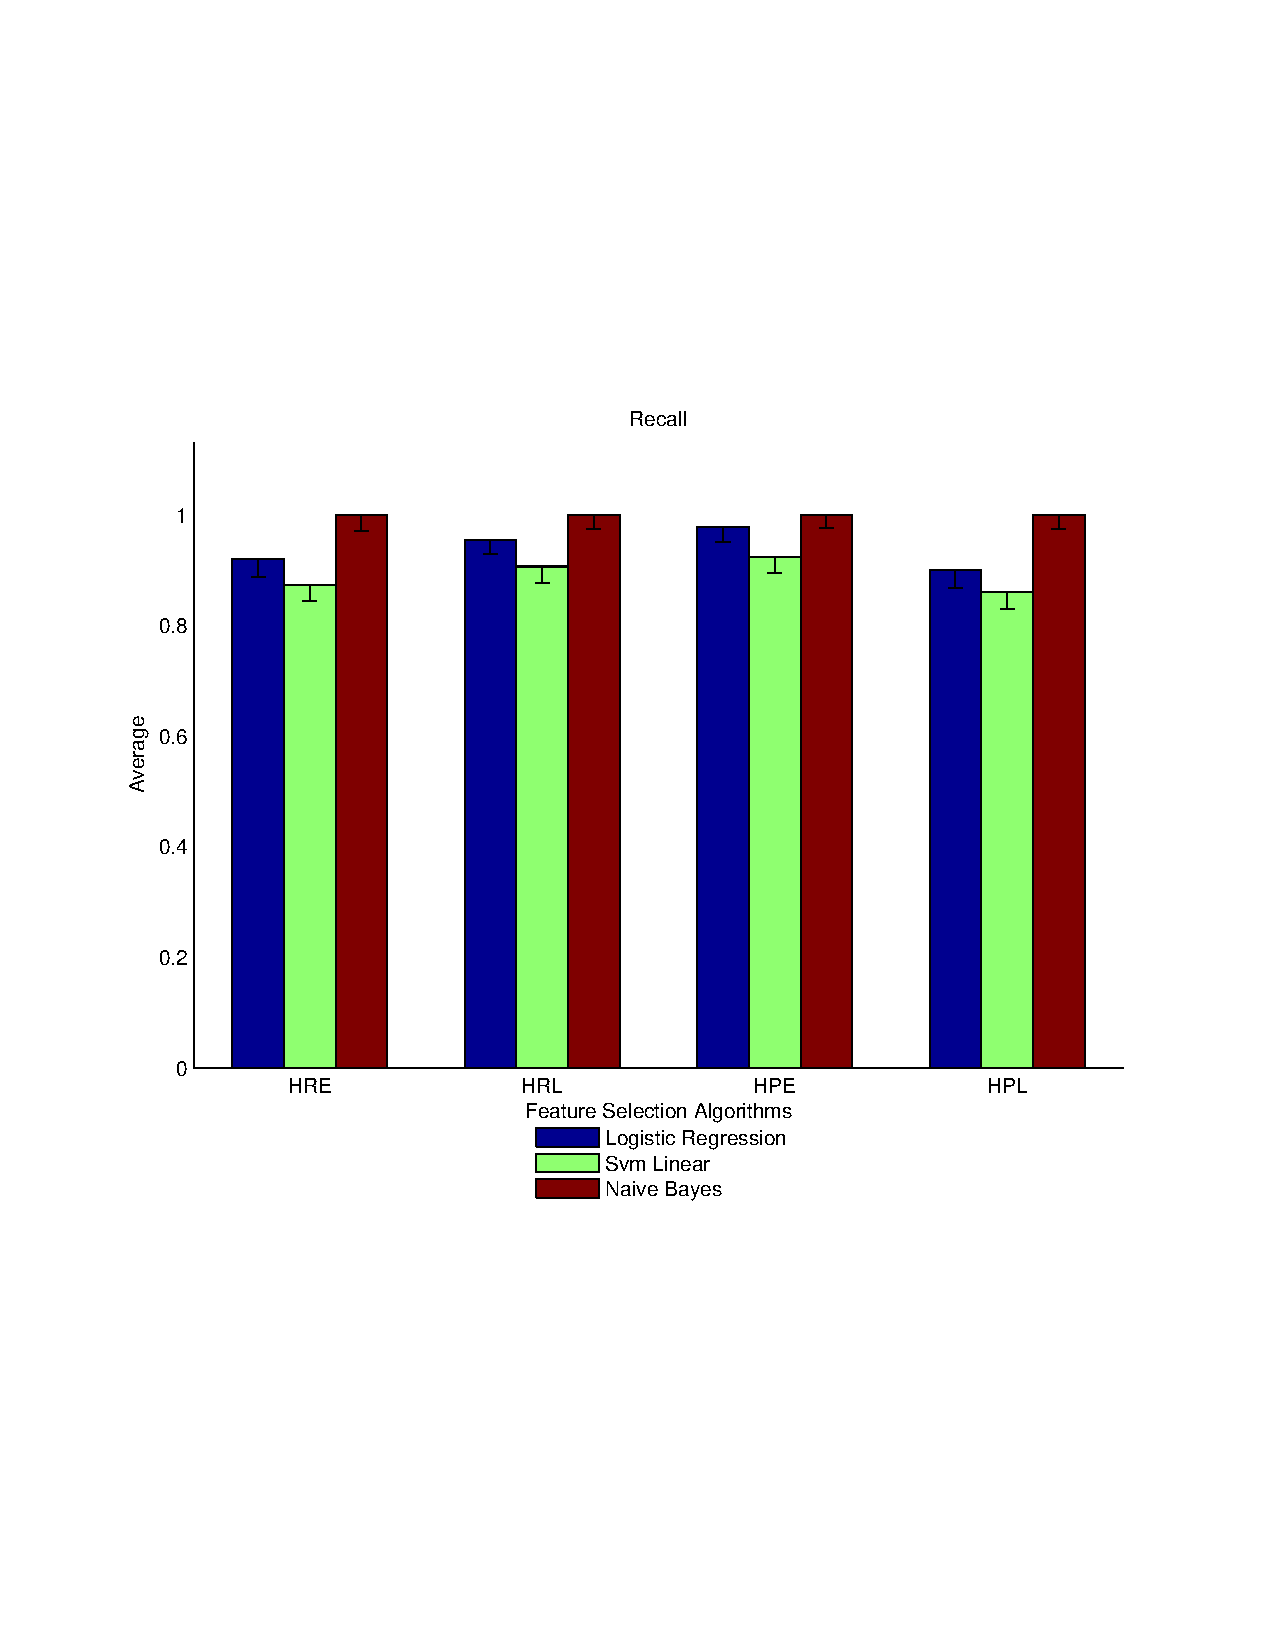
\includegraphics[width=0.35\textwidth]{../ResultsPlot/OthersDataSets/BarGraphs/bargraph4/Recall.pdf}
\caption{\footnotesize Performance of various feature selection algorithms per classifier, averaged across dataset and each stage of feature selection.}
\label{fig:perf_vs_classifier}
\end{figure*}
%%%%%%%%%%%%%%%%%%%%%%%%%%%%%%%%%%%%%%%%%%%%%%%%%%%%%%%%%%%%%%%%%%%%%%%%%%

%%%%%%%%%%%%%%%%%%%%%%%%%%%%%%%%%%%%%%%%%%%%%%%%%%%%%%%%%%%%%%%%%%%%%%%%%%
\begin{figure*}[tbp!]
\centering
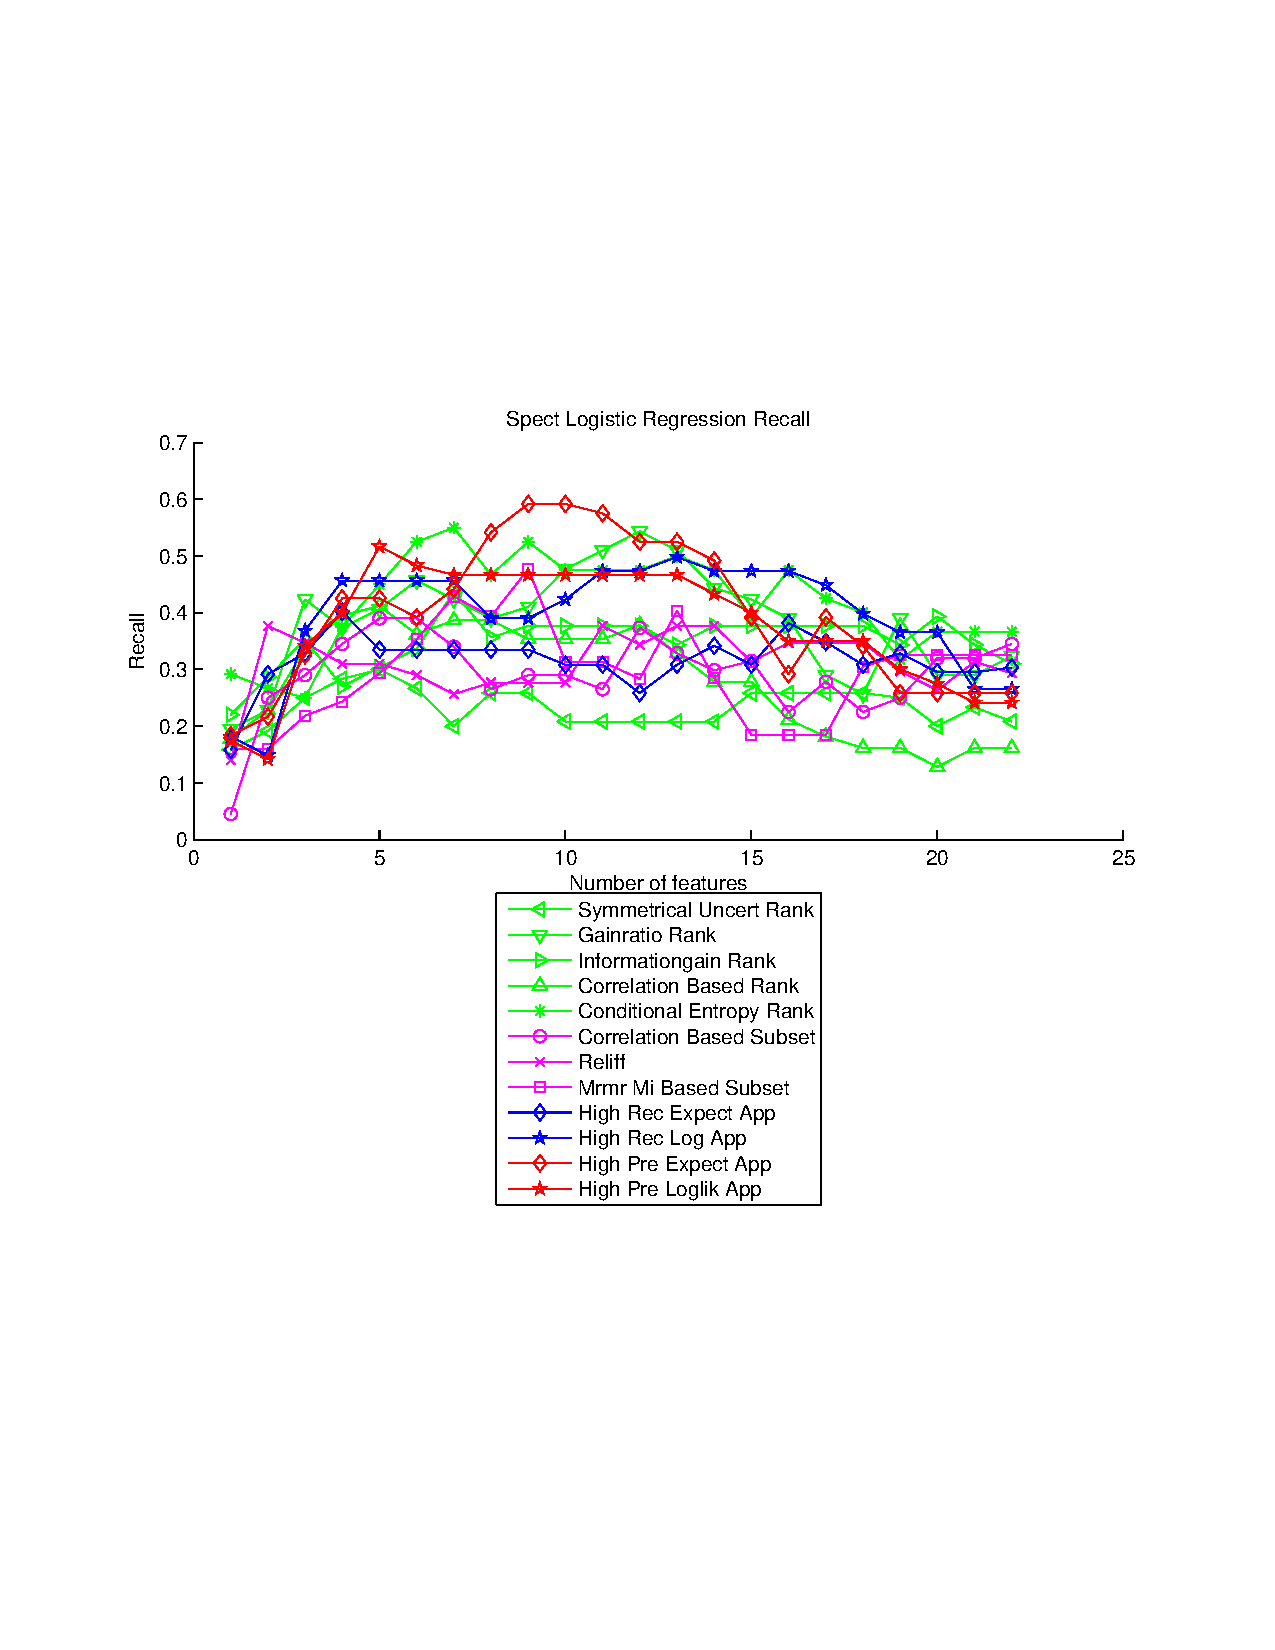
\includegraphics[width=0.35\textwidth]{../ResultsPlot/OthersDataSets/LineGraphs/FullResultsWithoutNoutOfK/Spect Logistic Regression Recall.pdf}
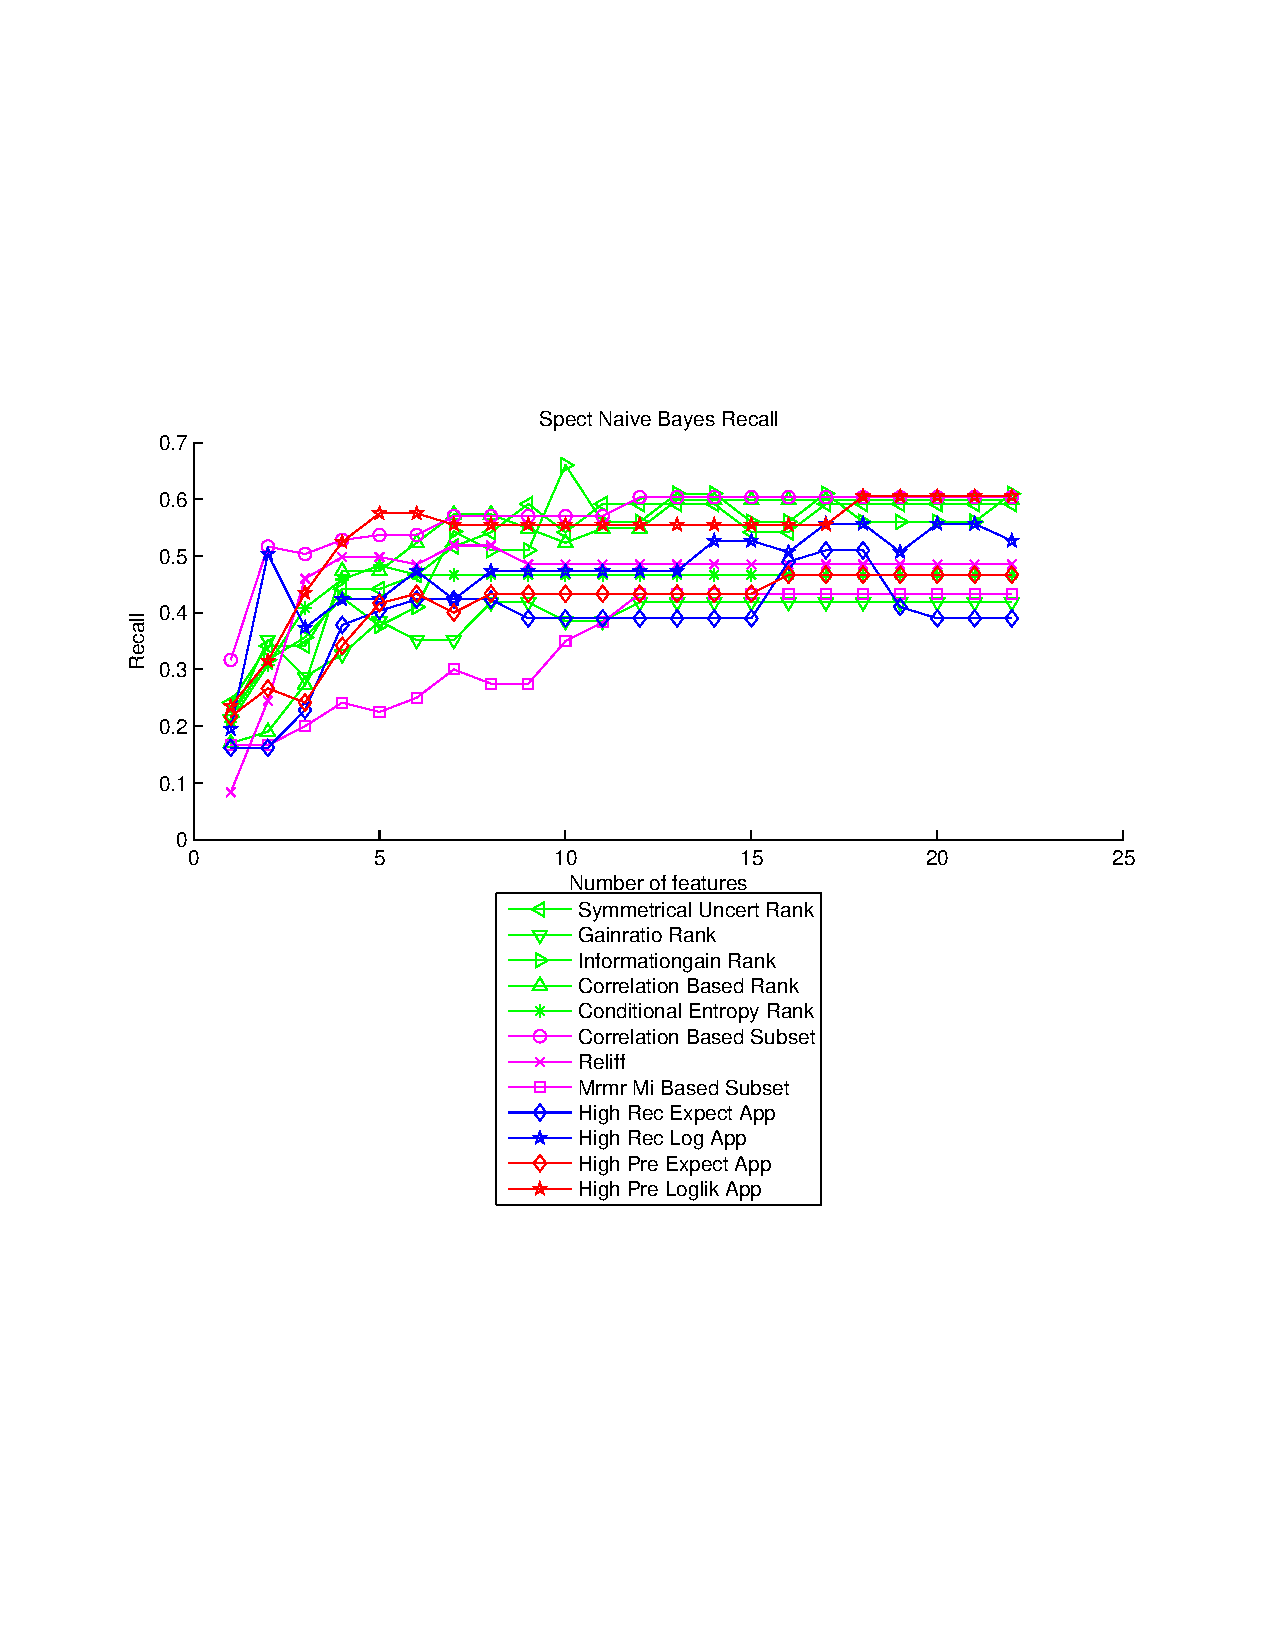
\includegraphics[width=0.35\textwidth]{../ResultsPlot/OthersDataSets/LineGraphs/FullResultsWithoutNoutOfK/Spect Naive Bayes Recall.pdf}\\
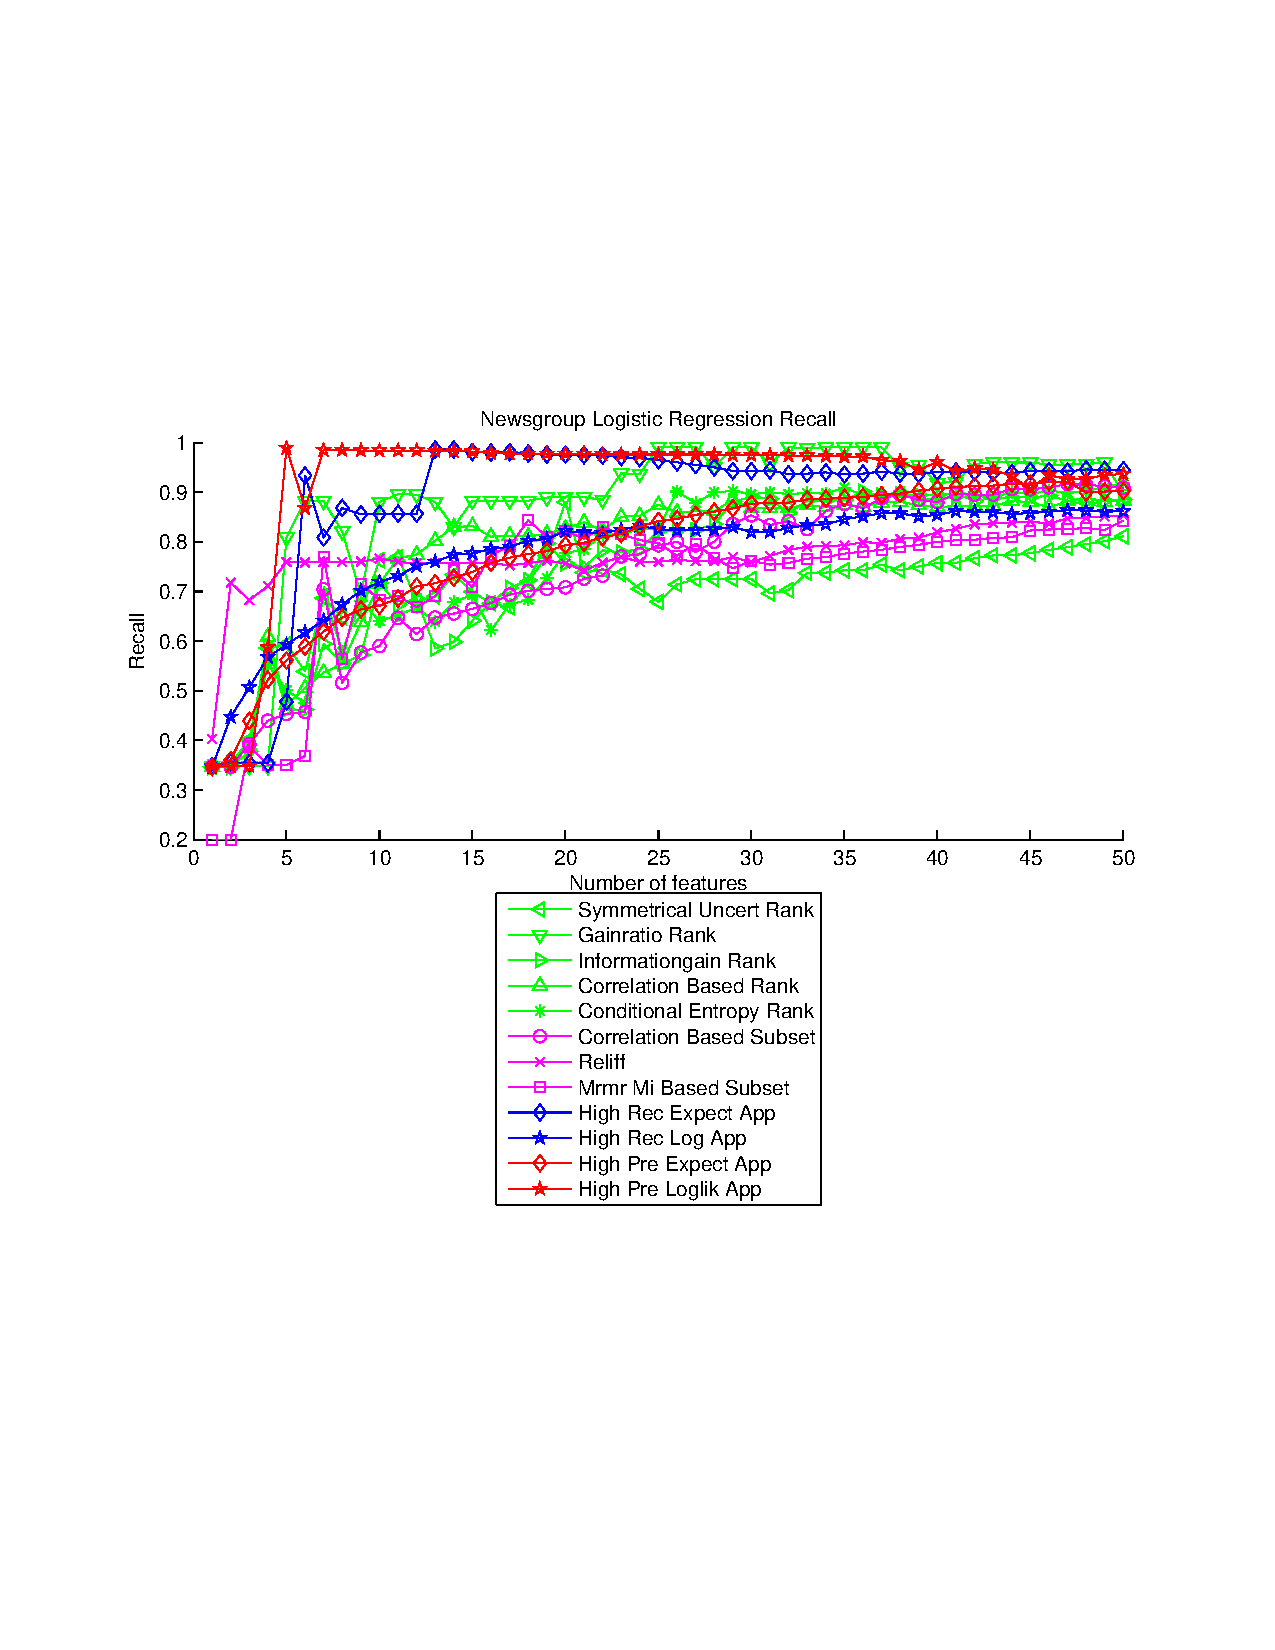
\includegraphics[width=0.35\textwidth]{../ResultsPlot/OthersDataSets/LineGraphs/FullResultsWithoutNoutOfK/Newsgroup Logistic Regression Recall.pdf}
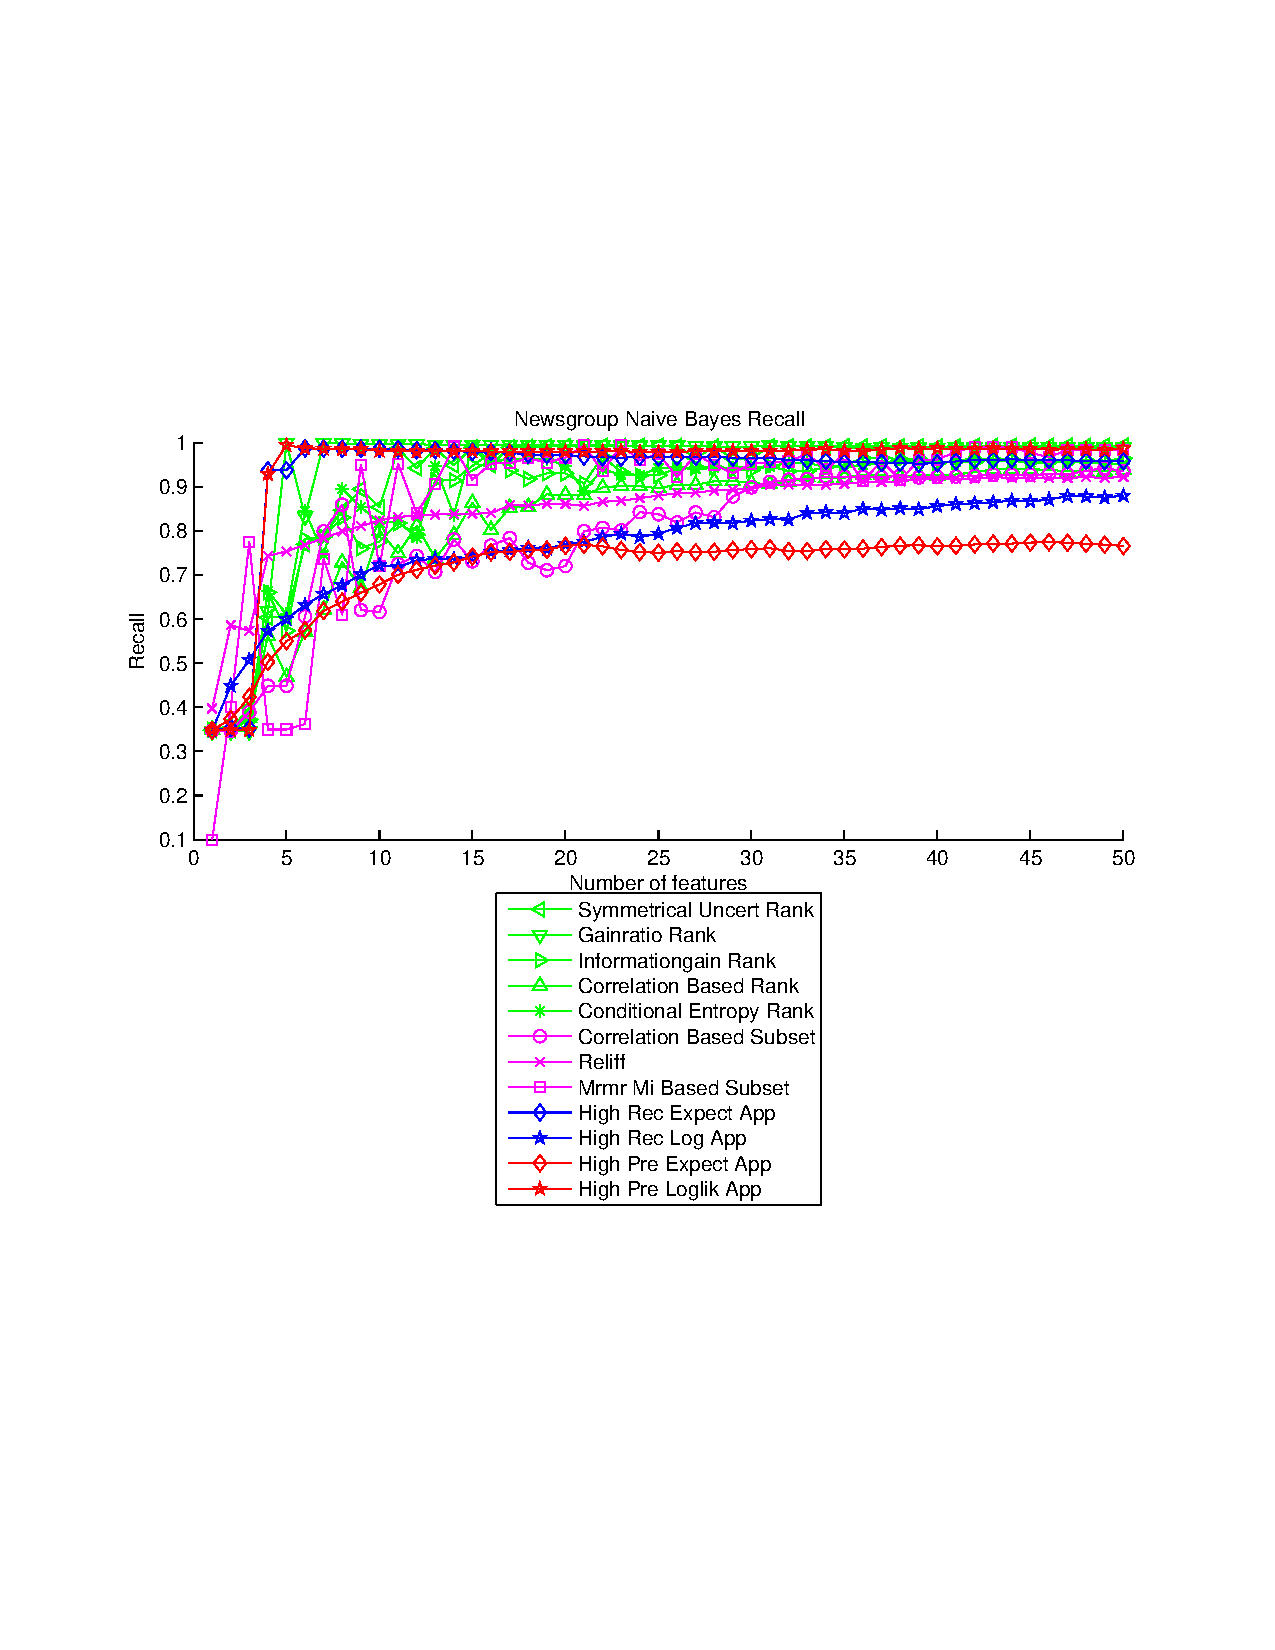
\includegraphics[width=0.35\textwidth]{../ResultsPlot/OthersDataSets/LineGraphs/FullResultsWithoutNoutOfK/Newsgroup Naive Bayes Recall.pdf}
\caption{\footnotesize Performance distribution of various feature selection algorithms with samples taken for each dataset, classifier type, and stage of feature selection.}
\label{fig:perf_vs_fs_alg}
\end{figure*}
%%%%%%%%%%%%%%%%%%%%%%%%%%%%%%%%%%%%%%%%%%%%%%%%%%%%%%%%%%%%%%%%%%%%%%%%%%

To answer these questions, we first start with
Figure~\ref{fig:perf_vs_dataset}, where we evaluate the performance of
various feature selection algorithms per dataset, averaged across
classifier type and each stage of feature selection.  We observe...
% TODO Scott

In Figure~\ref{fig:perf_vs_classifier}, we examine how well our 
novel feature selection algorithms HRE, HRL, HPE, HPL 
perform vs. classifier, noting that overall performance is best
for Naive Bayes followed by Logistic Regression and noticeably worse for
the SVM --- it seems simply that the probabilistic nature of our feature selection
dovetail best with classification methods that are themselves probabilistic,
and overall best with Naive Bayes which makes the same independence assumptions.
{\bf TODO Rodrigo: can we get bargraphs like those in FeatureSelection classifier,
except only showing HRE, HRL, HPE, HPL *and* averaging over all datasets?
So major group={HRE, HRL, HPE, HPL}, minor group={SVM,LR,NB} and one graph
for each of A/P/R/F.  Also the filename should not have spaces.}

Next we examine Figure~\ref{fig:perf_vs_fs_alg}, where we evaluate the
performance distribution of various feature selection algorithms with
samples taken for each dataset, classifier type, and stage of feature
selection.  Here we see Y.  We observe...

